\documentclass[aspectratio=169]{beamer}

% Load general definitions
\usepackage[utf8]{inputenc}
%\usepackage[T1]{fontenc}
\usepackage[brazil]{babel}
\usepackage{amsmath}
\usepackage{amsfonts}
\usepackage{amssymb}
\usepackage{graphicx}
\usepackage{verbatim}
\usepackage{cancel}
\usepackage{askmaps}
\usepackage{tabularx}
\usepackage[table]{xcolor}
%\usepackage{tikz}
\usepackage{multirow}
\usepackage{mathtools}
\usepackage{color, colortbl}
\usepackage{etoolbox}
\usepackage{pbox}
\usepackage{changepage}
\usepackage{xpatch}
\usepackage{array}
\usepackage{marvosym}
\usepackage{tabu}
\usepackage{multicol}
\usepackage{listings}
\usepackage{underscore}
\usepackage{filecontents}
\usepackage[]{algorithm2e}
\usepackage{ragged2e}

\newcolumntype{P}[1]{>{\centering\arraybackslash}m{#1}}
\definecolor{Gray}{gray}{0.75}
\definecolor{Gray2}{gray}{0.85}

\definecolor{lightBlue}{HTML}{DAE8FC}
\definecolor{Blue}{RGB}{51, 51, 204}

%\useinnertheme[lily]{rounded}
\usetheme{UniEvangelica}
%\usetheme{Copenhagen}
%\usetheme{Berlin}
%\usecolortheme{dolphin}
\tolerance=1
\emergencystretch=\maxdimen
\hyphenpenalty=10000
\hbadness=10000

\setbeamertemplate{navigation symbols}{}%remove navigation symbols


\let\olditem=\item% 
\renewcommand{\item}{\olditem \justifying}%
\def\center{\trivlist \centering\item\relax}
\def\endcenter{\endtrivlist}

\setbeamertemplate{itemize/enumerate body begin}{\large}
\setbeamertemplate{itemize/enumerate subbody begin}{\large}

\setbeamertemplate{itemize item}{\raisebox{0.1ex}{$\blacktriangleright$}\hskip0.1em}
\setbeamertemplate{itemize subitem}{\raisebox{0.1ex}{$\blacktriangleright$}\hskip0.1em}

\newcommand{\greenarrow}{\textcolor{green}{\rotatebox[origin=c]{180}{\MVArrowDown}}}

\newcommand{\redarrow}{\textcolor{red}{\MVArrowDown}}

%\newcommand{\ftable}{
%	\begin{table}
%		\large
%		\centering
%		\rowcolors{1}{\ifnumless{\rownum}{2}{Blue}{lightBlue}}{}
%}

\newenvironment{eftable}{
	\begin{table}
		\large
		\centering
		\rowcolors{1}{}{Blue}
		\rowcolors{1}{\ifnumless{\rownum}{2}{Blue}{lightBlue}}{}
	}
	{
	\end{table}
}


%\setbeamertemplate{frametitle}
%{
%	%\vspace*{-2em}	
%	\insertframetitle
%
%	 %\textcolor{white}{\LARGE \insertframetitle}
%
%}

% Specific definitions
\title[]{Sistemas Inteligentes}
\subtitle[]{Conceitos Fundamentais}
\author[]{Prof. Alexandre Tannus}
\date{}

\begin{document}

	\begin{frame}
		\titlepage
	\end{frame}

	\begin{frame}
		\tableofcontents		
	\end{frame}	
	
	\section{Introdução}
	
	\begin{frame}
		\frametitle{Questionamentos}
		\begin{itemize}
			\item O que é artificial? 

			\item O que é inteligência?

			\item O que é Inteligência artificial?

			\item Onde se aplica?

		\end{itemize}
	\end{frame}
	
	\begin{frame}
		\frametitle{O que é Inteligência Artificial?}
		\begin{itemize}
			\item Ramo da ciência da computação que se ocupa da automação do comportamento inteligente (Luger, 2004)

			\item Inteligência Artificial envolve utilizar métodos baseados no comportamento inteligente de humanos e outros animais para solucionar problemas complexos (Coppin, 2013)

		\end{itemize}
	\end{frame}	
	
	\begin{frame}
		\frametitle{O que é Inteligência Artificial?}
		\begin{itemize}
			\item De acordo com Russel (2004)
			\begin{itemize}
				\item Pensamento como seres humanos
				\item Pensamento racional
				\item Atuação como seres humanos
				\item Atuação racional				
			\end{itemize}
		\end{itemize}	
	\end{frame}
	
	\begin{frame}
		\frametitle{Pensamento humano}
		\begin{quote}
		"O novo e interessante esforço para fazer os computadores pensarem... Máquinas com mentes, no sentido total e literal" – Haugeland, 1985
		\end{quote}
		\begin{itemize}
			
			\item Modelagem cognitiva
			
			\item Necessário pesquisa científica bem fundamentada para avaliar o comportamento humano em determinadas situações
			
			\item General Problem Solver (Newell e Simon, 1961)
		
		\end{itemize}
	\end{frame}	

	\begin{frame}
		\frametitle{Pensando racionalmente}
		\begin{quote}
			"O estudo das faculdades mentais pelo uso de modelos computacionais" – Charniak e McDermott, 1985
		\end{quote}
		
		\begin{itemize}
			\item Silogismos, lógica clássica
		\end{itemize}
	\end{frame}

	\begin{frame}
		\frametitle{Agindo racionalmente}
		\begin{quote}
			"A Inteligência Computacional é o estudo de agentes inteligentes" – Poole et al., 1998
		\end{quote}
		
		\begin{itemize}
			\item Realizar ações para alcançar o melhor resultado possível e/ou esperado

			\item Pode incluir etapas de pensamento racional
		\end{itemize}
	\end{frame}

	\begin{frame}
		\frametitle{Agindo de forma humana}
		\begin{quote}
			"A arte de criar máquinas que executam funções que exigem inteligência quando executadas por pessoas" – Kurzweil, 1990
		\end{quote}
		
		\begin{itemize}
			\item Teste de Turing
			\begin{itemize}
				\item Distinção entre seres humanos e máquinas
			\end{itemize}
		\end{itemize}
	\end{frame}
	
	\begin{frame}
		\frametitle{Teste de Turing – Capacidades da máquina}
		\begin{itemize}
			\item Processamento de linguagem natural
			\begin{itemize}
				\item Entendimento do idioma falado pelo interlocutor
			\end{itemize}
			\item Representação do conhecimento
			\begin{itemize}
				\item Armazenamento das percepções do ambiente
			\end{itemize}
			\item Raciocínio automatizado
			\begin{itemize}
				\item Responder perguntas, realizar inferências e tirar conclusões
			\end{itemize}

		\end{itemize}
	\end{frame}	

	\begin{frame}
		\frametitle{Teste de Turing – Capacidades da máquina}
		\begin{itemize}
			\item Aprendizado de máquina
			\begin{itemize}
				\item Adaptação a novas situações e detecção de novos padrões
			\end{itemize}
			\item Visão computacional
			\begin{itemize}
				\item Percepção de objetos no ambiente
			\end{itemize}
			\item Robótica
			\begin{itemize}
				\item Manipulação de objetos e movimentação
			\end{itemize}

		\end{itemize}
	\end{frame}	

	\section{Fundamentos da I.A.}
	
	\begin{frame}
		\frametitle{Bases da I.A.}
		\begin{itemize}
			\item Filosofia
			\item Matemática
			\item Economia
			\item Neurociência
			\item Psicologia
			\item Engnharia da Computação
			\item Teoria de Controle
			\item Linguística			
		\end{itemize}
	\end{frame}	
	
	\begin{frame}
		\frametitle{Filosofia (428 a.C – hoje)}
		
		\begin{itemize}
			\item Regras formais podem ser utilizadas para a obtenção de conclusões válidas?

			\item De onde vem o conhecimento?

			\item Como utilizá-lo para determinar ações?

		\end{itemize}
	\end{frame}
	
	\begin{frame}
		\frametitle{Matemática (800 – hoje)}
		\begin{itemize}
			\item Quais regras formais podem ser utilizadas?
			
			\begin{table}
				\centering
				\begin{tabular}{c c}
					Álgebra booleana & Lógica de primeira  ordem	\\				
					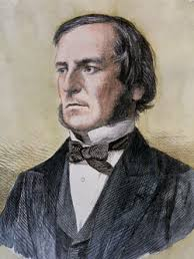
\includegraphics[height=4.5cm, keepaspectratio]{../figs/cap01/boole.png} 
					&
					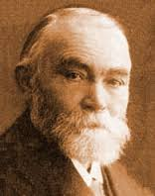
\includegraphics[height=4.5cm, keepaspectratio]{../figs/cap01/frege.png} \\
					George Boole & Gottlob Frege 
					
					
				\end{tabular}
			\end{table}
		\end{itemize}
	\end{frame}

	\begin{frame}
		\frametitle{Matemática (800 – hoje)}
		\begin{itemize}
			\item O que pode ser computado?
			\begin{itemize}
				\item Algoritmos
				\item David Hilbert (23 problemas que ocupariam os matemáticos)
				\item Kurt Gödel ( Teorema da incompleteza)
				\item Alan Turing (Máquina de Turing)
				\item Avaliação de complexidade (década de 60)
				\item Problemas NP-Completos (Cook, 1971; Karp, 1972)			
			\end{itemize}
		\end{itemize}
	\end{frame}

	\begin{frame}
		\frametitle{Matemática (800 – hoje) - Incertezas}
		\begin{itemize}
			\item Probabilidade			
			
			\begin{table}
				\centering
				\begin{tabular}{c}
					Jogos de azar \\				
					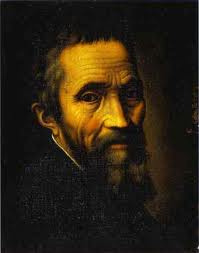
\includegraphics[height=4.5cm, keepaspectratio]{../figs/cap01/cardano.jpg} \\
					Gerolamo Cardano  		
					
				\end{tabular}
			\end{table}
		\end{itemize}
	\end{frame}

	\begin{frame}
		\frametitle{Matemática (800 – hoje) - Incertezas}
		\begin{itemize}
			\item Aperfeiçoamento da teoria e métodos estatísticos
			

		\end{itemize}

		
		\begin{adjustwidth}{-2.5em}{-2em}
			\begin{table}
				\centering
				\begin{tabular}{c c c c}				
					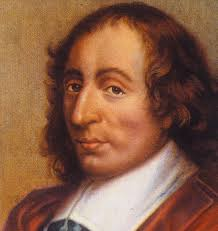
\includegraphics[height=3.5cm, keepaspectratio]{../figs/cap01/pascal.jpg} &				
					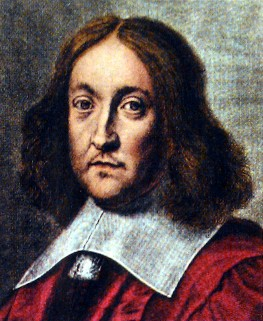
\includegraphics[height=3.5cm, keepaspectratio]{../figs/cap01/fermat.jpg} &				
					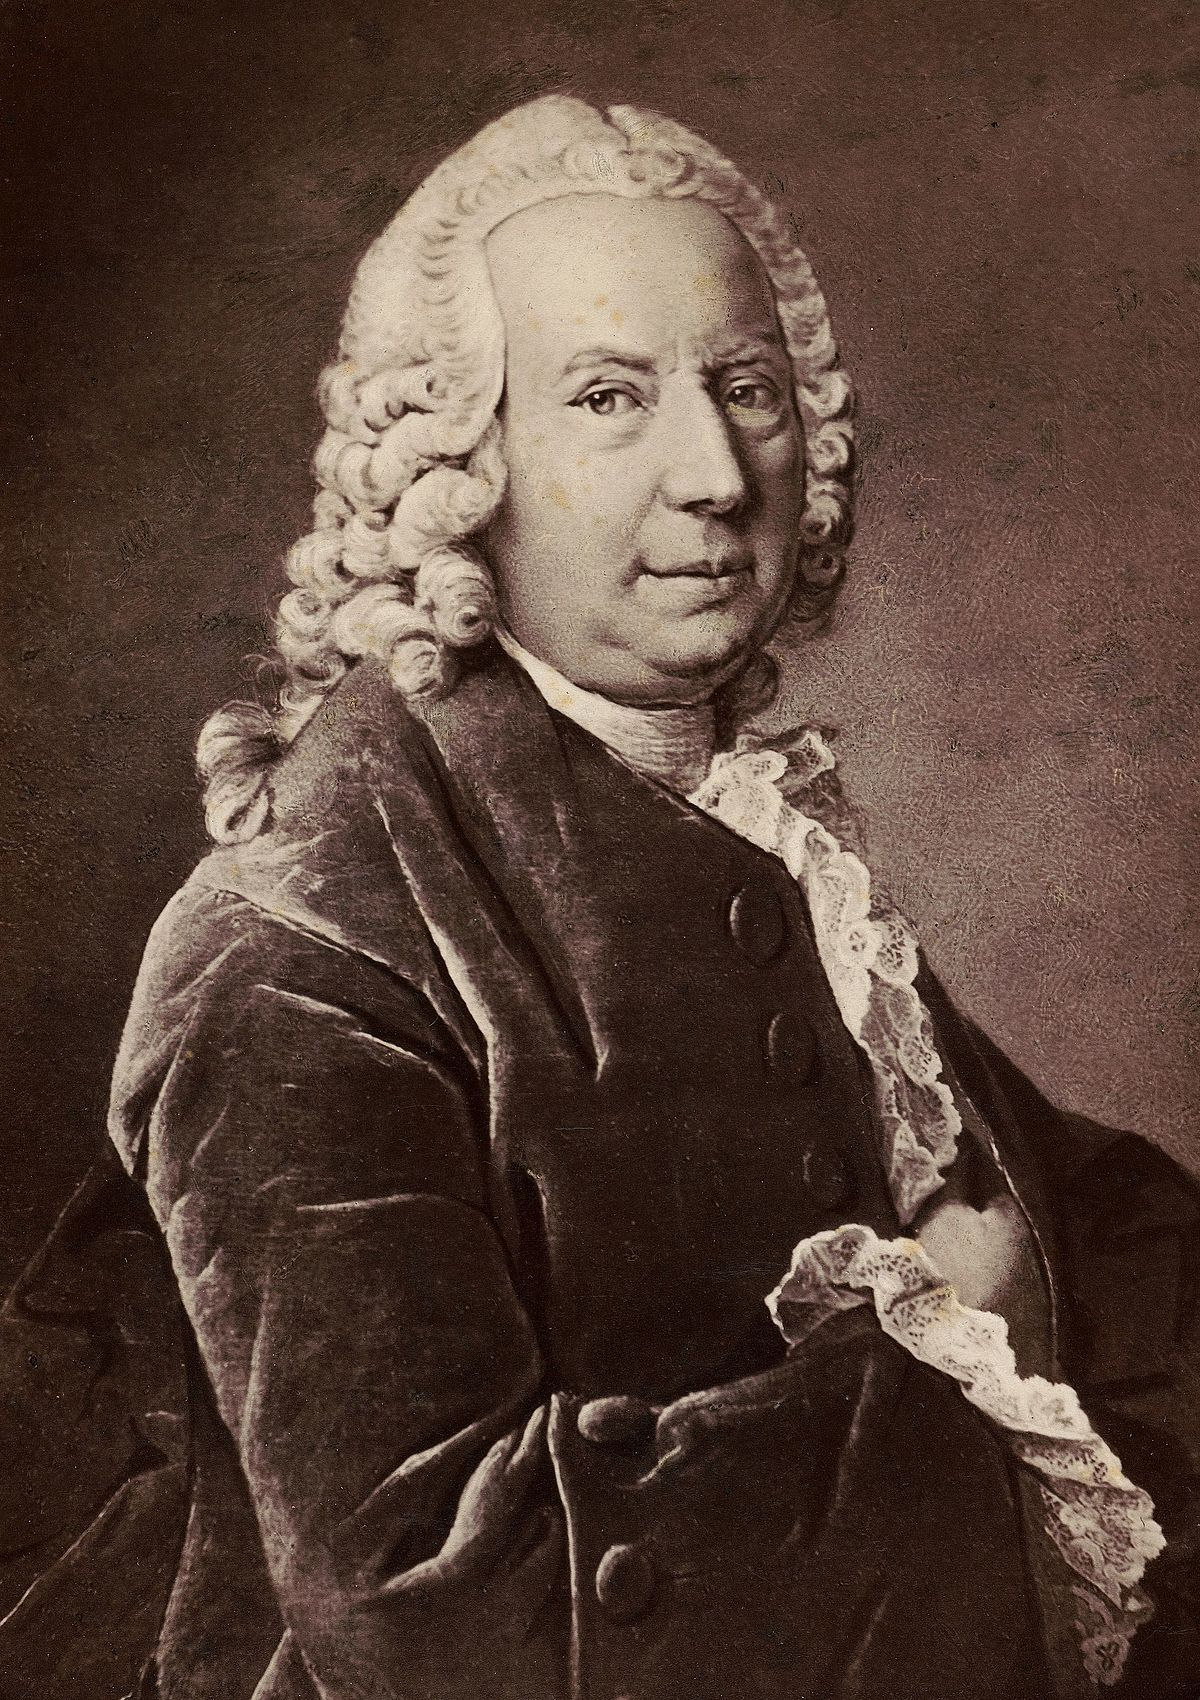
\includegraphics[height=3.5cm, keepaspectratio]{../figs/cap01/bernoulli.jpg} &				
					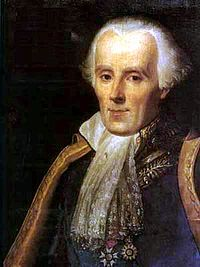
\includegraphics[height=3.5cm, keepaspectratio]{../figs/cap01/laplace.jpg} 
					\\
					Pascal & Fermat & Bernoulli & Laplace 		
					
				\end{tabular}
			\end{table}		
		\end{adjustwidth}		
		
	\end{frame}

	\begin{frame}
		\frametitle{Matemática (800 – hoje) - Incertezas}
		\begin{itemize}
			\item Regras Bayesianas
			\begin{itemize}
				\item Base das teorias de incerteza em IA
			\end{itemize}
		\end{itemize}
		
			\begin{table}
				\centering
				\begin{tabular}{c}				
					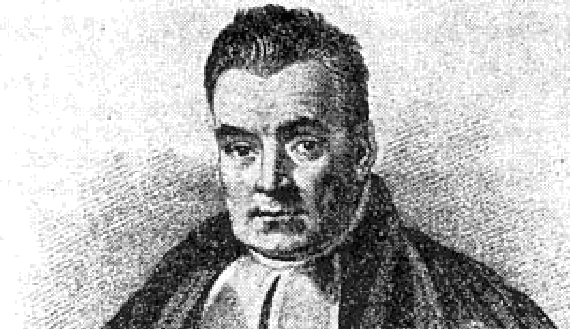
\includegraphics[height=4.5cm, keepaspectratio]{../figs/cap01/bayes.png} \\
					Thomas Bayes 		
					
				\end{tabular}
			\end{table}
							
	\end{frame}

	\begin{frame}
		\frametitle{Economia (1776 – hoje)}
		\begin{itemize}
			\item É possível maximizar o lucro
			\begin{itemize}
				\item Adam Smith (pai da economia)
				\item Teoria da utilidade (Leon Walras, Frank Ramsey, Von Neumann, Morgenstern)
			\end{itemize}
			\item Como conciliar isso com as pessoas e o tempo?
			\begin{itemize}
				\item Probabilidade + utilidade = Teoria da decisão (teoria dos jogos)
				\item Pesquisa operacional
				\item Processos de decisão de Markov
				\item Modelos baseados em satisfação
			
			\end{itemize}
		\end{itemize}
	\end{frame}
	
	\begin{frame}
		\frametitle{Neurociência (1861 – hoje)}
		\begin{quote}
			“Embora um computador seja um milhão de vezes mais rápido em velocidade de comutação bruta, o cérebro acaba sendo 100 mil vezes mais rápido no que faz” – Russel, 2004
		\end{quote}
	\end{frame}
	
	\begin{frame}
		\frametitle{Neurociência (1861 – hoje)}
		\begin{itemize}
			\item Como o cérebro processa as informações? 
		\end{itemize}
					\begin{table}
				\centering
				\begin{tabular}{c c c}	
					Áreas cerebrais & Visualização dos neurônios & EEG			\\
					1861 & 1873 & 1929 \\
					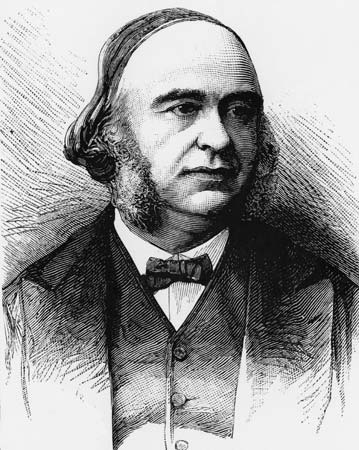
\includegraphics[height=3.5cm, keepaspectratio]{../figs/cap01/broca.jpg} &				
					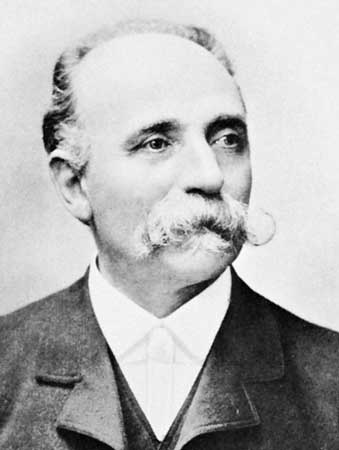
\includegraphics[height=3.5cm, keepaspectratio]{../figs/cap01/golgi.jpg} &				
					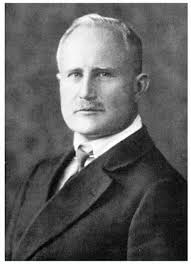
\includegraphics[height=3.5cm, keepaspectratio]{../figs/cap01/berger.jpg}  
					\\
					Paul Broca & Camilo Golgi & Hans Berger 		
					
				\end{tabular}
			\end{table}
	\end{frame}	
	
	\begin{frame}
		\frametitle{Psicologia (1874 – hoje)}
		\begin{itemize}
			\item Como é o pensamento e a ação de animais e humanos?
			\begin{itemize}
				\item Ciência cognitiva
				\item Behaviorismo
				\begin{itemize}
					\item Medidas objetivas de percepção e ações resultantes

				\end{itemize}
			\end{itemize}
		\end{itemize}
		
		\begin{table}
			\centering
			\begin{tabular}{c}				
				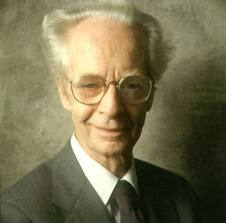
\includegraphics[height=4.5cm, keepaspectratio]{../figs/cap01/skinner.jpg} \\
				B.F. Skinner 		
				
			\end{tabular}
		\end{table}
	\end{frame}	

	\begin{frame}
		\frametitle{Engenharia de Computação (1940 – hoje)}
		\begin{itemize}
			\item Como construir computadores eficientes?
			\begin{itemize}
				\item Alan Turing
				\begin{itemize}
					\item Primeiro computador operacional
					\item Decifrador de mensagens alemãs
					\item Jogo da Imitação (2014)

				\end{itemize}
			\end{itemize}
		\end{itemize}
		
		\begin{table}
			\centering
			\begin{tabular}{c}				
				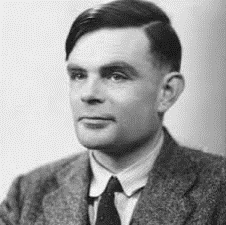
\includegraphics[height=4.5cm, keepaspectratio]{../figs/cap01/turing.png} \\		
				
			\end{tabular}
		\end{table}
	\end{frame}

	\begin{frame}
		\frametitle{Engenharia de Computação (1940 – hoje)}
		\begin{itemize}
			\item Como construir computadores eficientes?
			\begin{itemize}
				\item Konrad Zuse
				\begin{itemize}
					\item Primeiro computador programável (Z-3)
					\item Criador da primeira linguagem (Plankalkül)
					\item Ponto flutuante
				\end{itemize}
			\end{itemize}
		\end{itemize}
		
		\begin{table}
			\centering
			\begin{tabular}{c}				
				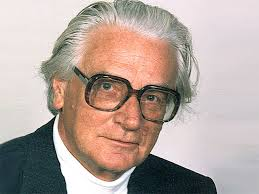
\includegraphics[height=4.5cm, keepaspectratio]{../figs/cap01/zuse.png} \\		
				
			\end{tabular}
		\end{table}
	\end{frame}

	\begin{frame}
		\frametitle{Engenharia de Computação (1940 – hoje)}
		\begin{itemize}
			\item Como construir computadores eficientes?
			\begin{itemize}
				\item John Mauchly e John Eckert
				\begin{itemize}
					\item ENIAC
					\item Projeto militar americano
				\end{itemize}
			\end{itemize}
		\end{itemize}
		
		\begin{table}
			\centering
			\begin{tabular}{c}				
				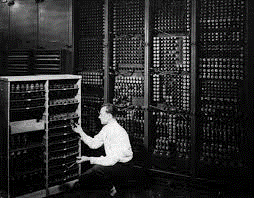
\includegraphics[height=4.5cm, keepaspectratio]{../figs/cap01/eniac.png} \\		
				
			\end{tabular}
		\end{table}
	\end{frame}

	\begin{frame}
		\frametitle{Teoria de controle (1948 – hoje)}
		\begin{itemize}
			\item Artefatos podem operar sem interferência humana?
			\begin{itemize}
				\item Norbert Wiener (Teoria de controle)
				\item Definição de função objetivo
				\begin{itemize}
					\item Minimização de erros
				\end{itemize}
			\end{itemize}
		\end{itemize}
		
		\begin{table}
			\centering
			\begin{tabular}{c}				
				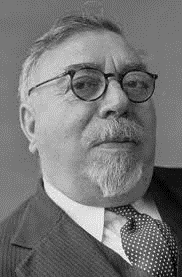
\includegraphics[height=4.5cm, keepaspectratio]{../figs/cap01/wiener.png} \\		
				
			\end{tabular}
		\end{table}
	\end{frame}

	\begin{frame}
		\frametitle{Linguística (1957 – hoje)}
		\begin{itemize}
			\item Noam Chomsky, 1957
			\begin{itemize}
				\item Formalização dos conceitos de linguagem natural
				\item Crítica à obra de B.F. Skinner (behaviorismo)
			\end{itemize}
			\item Processamento de linguagem natural
			\begin{itemize}
				\item Compreensão do assunto e do contexto
			\end{itemize}
		\end{itemize}
		
		\begin{table}
			\centering
			\begin{tabular}{c}				
				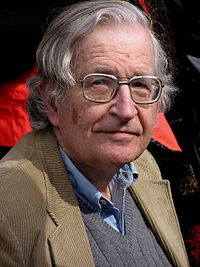
\includegraphics[height=4.5cm, keepaspectratio]{../figs/cap01/chomsky.jpg} \\		
				
			\end{tabular}
		\end{table}
	\end{frame}
	
	\section{História da I.A}

	\begin{frame}
		\frametitle{O início da I.A (anos 40)}
		\begin{itemize}
			\item Warren McCulloch e Walter Pitts (1943)
			\begin{itemize}
				\item Redes neurais
				\item Conhecimento de fisiologia
				\item Análise de lógica proposicional
				\item Teoria da computação
				\item Qualquer função computável pode ser calculada por uma rede de neurônios conectados
			\end{itemize}
		\end{itemize}
		
		\begin{table}
			\centering
			\begin{tabular}{c c}				
				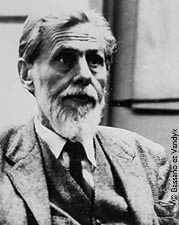
\includegraphics[height=3cm, keepaspectratio]{../figs/cap01/wsmcculloch.jpg} & 				
				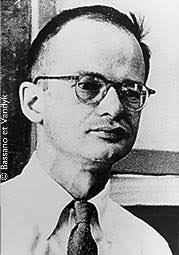
\includegraphics[height=3cm, keepaspectratio]{../figs/cap01/pitts.jpg} \\	
				Warren McCulloch & Walter Pitts
				
			\end{tabular}
		\end{table}
	\end{frame}	

	\begin{frame}
		\frametitle{O início da I.A (anos 40)}
		\begin{itemize}
			\item Donald Hebb (1949)
			\begin{itemize}
				\item Aprendizagem da rede neural
				\item Regra de atualização das intensidades de conexões 
			\end{itemize}
		\end{itemize}
		
		\begin{table}
			\centering
			\begin{tabular}{c}				
				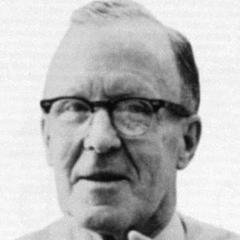
\includegraphics[height=3cm, keepaspectratio]{../figs/cap01/hebb.jpg} 
				
			\end{tabular}
		\end{table}
	\end{frame}	

	\begin{frame}
		\frametitle{Nascimento da I.A.}
		\begin{itemize}
			\item Seminário em Dartmouth (1956)


		\end{itemize}
		\begin{adjustwidth}{-2.5em}{-2em}
			\begin{table}
				
				\centering
				\begin{tabular}{c c c c c}				
					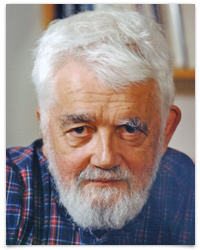
\includegraphics[height=3cm, keepaspectratio]{../figs/cap01/mccarthy.jpg} & 				
					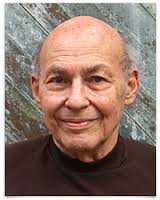
\includegraphics[height=3cm, keepaspectratio]{../figs/cap01/minsky.jpg} & 				
					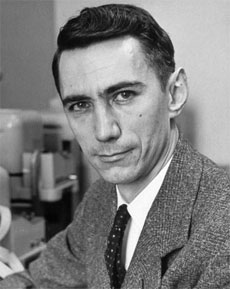
\includegraphics[height=3cm, keepaspectratio]{../figs/cap01/shannon.jpg}& 				
					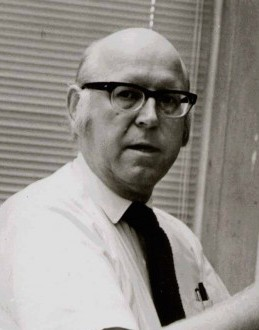
\includegraphics[height=3cm, keepaspectratio]{../figs/cap01/newell.jpg}& 				
					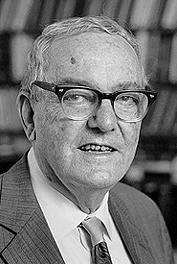
\includegraphics[height=3cm, keepaspectratio]{../figs/cap01/simon.jpg}\\	
					John McCarthy & Marvin Minsky & Claude Shannon & Allen Newell & Herbert Simon
					
				\end{tabular}
			\end{table}		
		\end{adjustwidth}

	\end{frame}	

	\begin{frame}
		\frametitle{Primeiros anos (1956 – 1969)}
		\begin{itemize}
			\item Dominados pelos participantes do seminário de Dartmouth e seus alunos
			\item John McCarthy (1958)
			\begin{itemize}
				\item LISP
				\item \textit{Advice Taker}
			\end{itemize}
			\item \textit{General Problem Solver} (1961)

		\end{itemize}
	\end{frame}

	\begin{frame}
		\frametitle{Choque de realidade}
		\begin{itemize}
			\item Desempenho promissor em problemas simples
			\begin{itemize}
				\item Redes neurais são limitadas
			\end{itemize}

			\item Problemas mais complexos não eram resolvidos de forma satisfatória
			\begin{itemize}
				\item Exemplo: tradução de textos
			\end{itemize}

			\item Início dos algoritmos genéticos
			
			\item Explosão combinatória
			
			\item Fim do apoio britânico às pesquisas em I.A. (1973)
		\end{itemize}
	\end{frame}

	\begin{frame}
		\frametitle{Sistemas especialistas (anos 70)}
		\begin{itemize}
			\item Desenvolvimento de sistemas para realizar operações específicas
			\begin{itemize}
				\item DENDRAL (análise molecular)
				\item MYCIN (diagnóstico de infecções sanguíneas)
				\item SHRDLU (linguagem natural)			
			\end{itemize}
		\end{itemize}
	\end{frame}

	\begin{frame}
		\frametitle{Indústria da I.A. (1980 – hoje)}
		\begin{itemize}
			\item Investimento governamental
			
			\item Retomada de pesquisas ‘esquecidas’
			
			\item Modelos ocultos de Markov
			
			\item Mineração de dados
			
			\item Redes bayesianas
			
			\item Agentes inteligentes		
		\end{itemize}
	\end{frame}

	\begin{frame}
		\frametitle{Questionamentos finais}
		\begin{itemize}
			\item O que é inteligência artificial?
			
			\item Os critérios de Turing são ideais para definir um sistema inteligente? Quais outros critérios seriam interessantes?
			
			\item É possível que um computador compreenda e utilize a linguagem humana?
			
			\item Quais são os pontos positivos e negativos do desenvolvimento da I.A  para a sociedade			
		\end{itemize}
	\end{frame}
		
	%Último slide
	\begin{frame}

	\end{frame}
\end{document}
